\documentclass[11pt,a4paper]{article}

% -------------------------------------------------
% PACKAGES
% -------------------------------------------------
\usepackage[utf8]{inputenc}
\usepackage[T1]{fontenc}
\usepackage[english]{babel}

\usepackage{geometry}
\geometry{left=2.5cm,right=2.5cm,top=2.5cm,bottom=2.5cm}

\usepackage{graphicx}
\usepackage{float}
\usepackage{hyperref}
\usepackage{booktabs}
\usepackage{longtable}
\usepackage{enumitem}
\usepackage{xcolor}
\usepackage{caption}
\usepackage{geometry}
\geometry{left=1.7cm,right=1.7cm,top=1.8cm,bottom=1.8cm}

\usepackage{listings}
\lstset{
  basicstyle=\ttfamily\small,
  breaklines=true,
  frame=single,
  numbers=left,
  numberstyle=\tiny,
  keywordstyle=\color{blue},
  commentstyle=\color{gray},
  stringstyle=\color{teal},
  showstringspaces=false
}

% -------------------------------------------------
% DOCUMENT INFO
% -------------------------------------------------
\title{\textbf{HandGesturesBot} \\ Project Documentation}
\author{HandGesturesBot \\ Mobile Embedded and Development / Hochschule Aalen}
\date{\today}

% -------------------------------------------------
% BEGIN DOCUMENT
% -------------------------------------------------
\begin{document}

\maketitle
\thispagestyle{empty}
\vspace{1cm}

\begin{center}
\textbf{Repository:} \href{https://github.com/notWetro/HandGestures2Bot.git}{HandGestures2Bot on GitHub}
\end{center}

\newpage
\tableofcontents
\newpage

% =================================================
% 1. PROJECT OVERVIEW AND GOAL
% =================================================
\section{Project Overview and Goal}
HandGestures2Bot is a project that enables controlling a TurtleBot robot using hand gestures captured via a mobile application.
The main goal is to provide an intuitive and modern way of robot control without traditional controllers, by using gesture recognition and network communication.

\subsection{Goal of the Project}
The main objectives of this project are:
\begin{itemize}[leftmargin=1.5cm]
    \item Provide a gesture-based robot control mechanism.
    \item Enable an easy setup process for connecting the robot and the mobile app.
    \item Ensure the system works reliably in a real environment (WiFi + Bluetooth provisioning).
    \item Keep the interaction focused on user experience and usability.
\end{itemize}

\subsection{Context Diagram / System Boundary}
This project connects a Flutter mobile app (gesture + voice control) with a TurtleBot3 running ROS~2.
The app sends movement commands via WebSocket over Wi-Fi. On the robot side, a safety scanner filters
the commands using LiDAR data and publishes safe velocity commands to the robot motors.
A Bluetooth provisioning service is used to configure the robot Wi-Fi and send the robot IP address back to the app.

\begin{figure}[H]
	\centering
	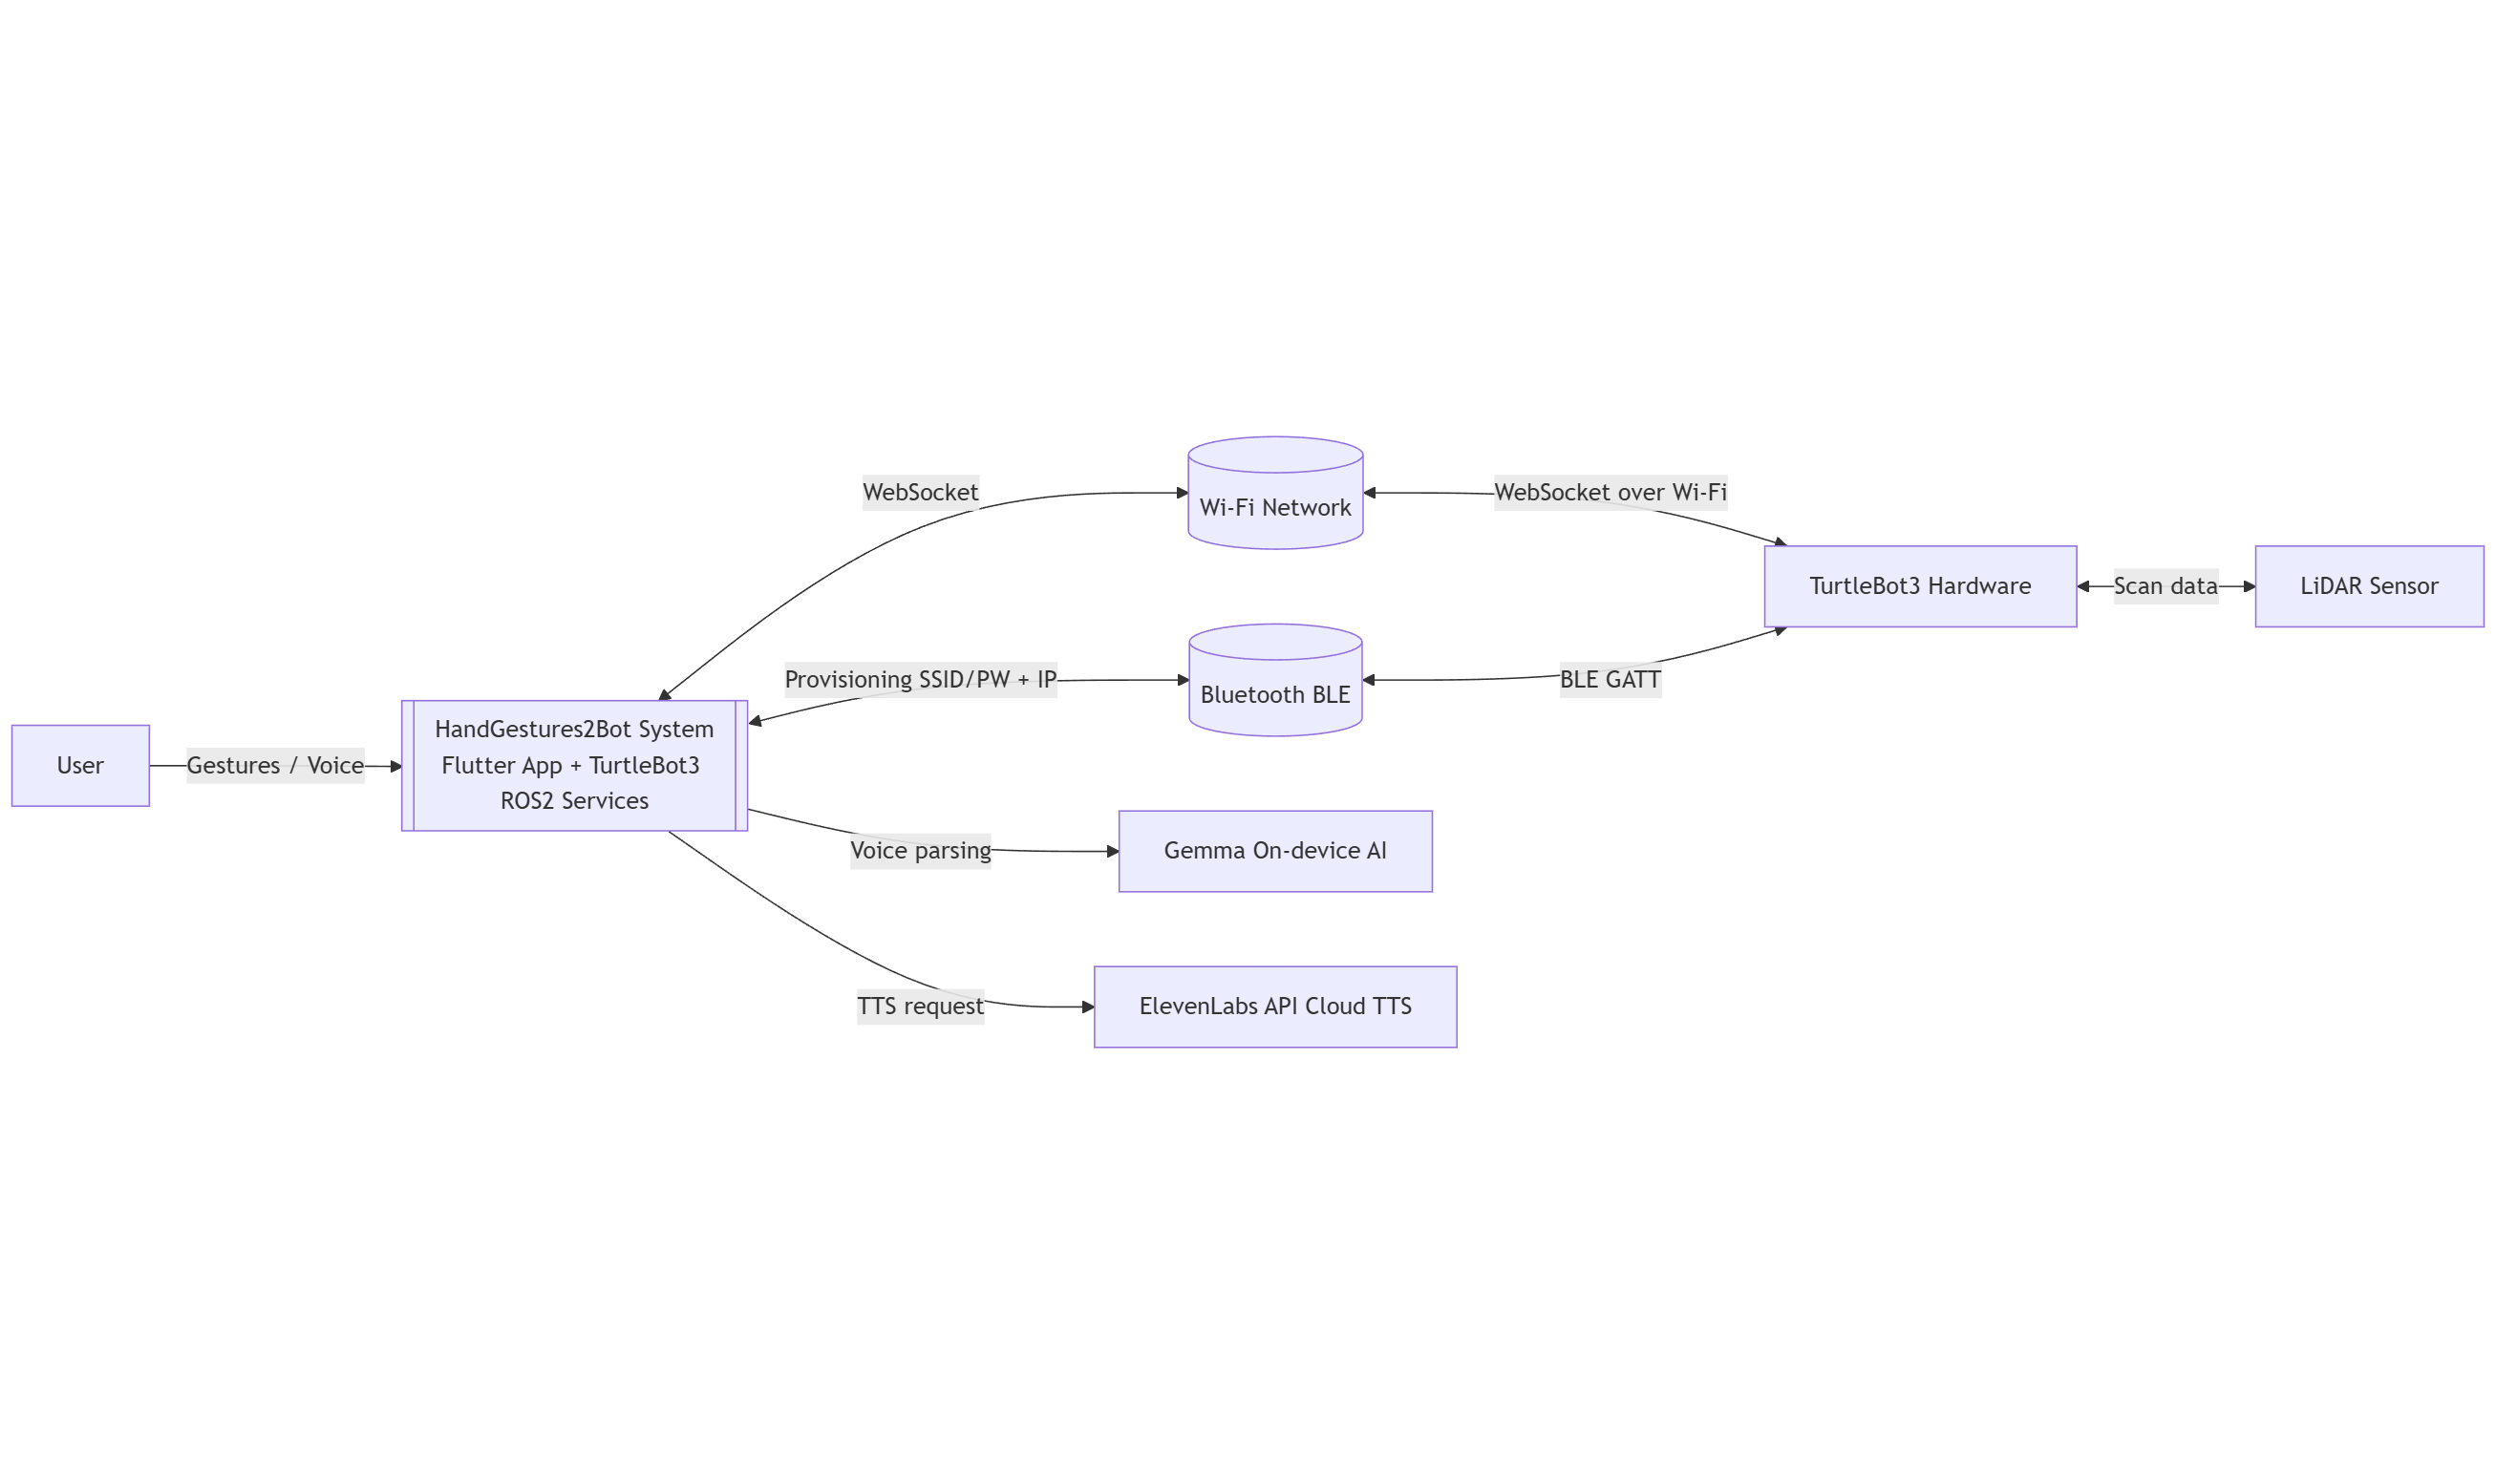
\includegraphics[width=1\textwidth]{figures/context_diagram_placeholder.png}
	\caption{Context Diagram (System Boundary)}
\end{figure}



\newpage
\subsubsection{External actors / environment}
\begin{itemize}[leftmargin=1.5cm]
	\item User (gesture + voice interaction)
	\item Wi-Fi network (WebSocket communication)
	\item Bluetooth Low Energy (Wi-Fi provisioning)
	\item TurtleBot3 hardware (motors + sensors) / LiDAR sensor (obstacle detection)
	\item ElevenLabs API (cloud TTS) / On-device AI model for voice command parsing
\end{itemize}

\subsubsection{Main interactions:}
\begin{itemize}[leftmargin=1.5cm]
	\item User $\rightarrow$ Flutter App: controls robot via gestures/voice
	\item Flutter App $\rightarrow$ Robot: sends \texttt{\{"movement": "..."\}} via WebSocket
	\item Robot $\rightarrow$ Flutter App: sends obstacle status updates
	\item Flutter App $\leftrightarrow$ Robot (BLE): sends Wi-Fi credentials and receives robot IP
\end{itemize}



% =================================================
% 2. FEATURES AND CAPABILITIES
% =================================================

\section{Features and Capabilities}

This section provides a high-level overview of the main features implemented in the HandGestures2Bot project.
Detailed scenarios and interaction flows are described in the next section.

\begin{itemize}[leftmargin=1.5cm]
	
	\item \textbf{Hand-gesture based robot control (Android):}
	Real-time gesture recognition using the camera and MediaPipe.
	
	\item \textbf{Voice-based robot control:}
	Speech-to-text, AI command interpretation, and optional TTS feedback.
	
	\item \textbf{Real-time robot control via WebSocket over Wi-Fi:}
	Sends JSON movement commands to the TurtleBot (\texttt{ws://<robot-ip>:8765}).
	
	\item \textbf{Supported movement commands:}
	Forward, backward, left, right, stop (unknown commands fall back to stop).
	
	\item \textbf{Safety obstacle filtering using LiDAR:}
	Blocks unsafe forward motion and prevents collisions.
	
	\item \textbf{Live obstacle status feedback to the mobile app:}
	Obstacle status updates are streamed back via WebSocket.
	
	\item \textbf{Bluetooth Low Energy (BLE) Wi-Fi provisioning:}
	Sends SSID/password and receives the robot IP address for Wi-Fi control.
	
	\item \textbf{Dance sequences / multi-step routines:}
	Gestures can trigger predefined movement sequences.
	
\end{itemize}

\newpage
% =================================================
% 3. SCENARIO AND FUNCTIONALITY DESCRIPTION
% =================================================
\section{Scenario and Functionality Description}

This section describes how the system is used across the system boundary.
The focus is on interactions between user/app/robot/network and not on internal architecture.

\subsection{Scenario 1: User controls the TurtleBot with Hand Gestures}
\textbf{Goal:} The user moves the TurtleBot using hand gestures detected by the mobile device.

\textbf{Actors:} User, Mobile App, TurtleBot

\textbf{Basic Flow:}
\begin{enumerate}[leftmargin=1.5cm]
    \item User opens the mobile app.
    \item The app activates gesture recognition using the device camera.
    \item Detected gestures are translated into movement commands.
    \item Commands are sent to the TurtleBot via WiFi.
    \item The TurtleBot executes movement (e.g., forward, left, right, stop).
\end{enumerate}

\begin{figure}[H]
    \centering
    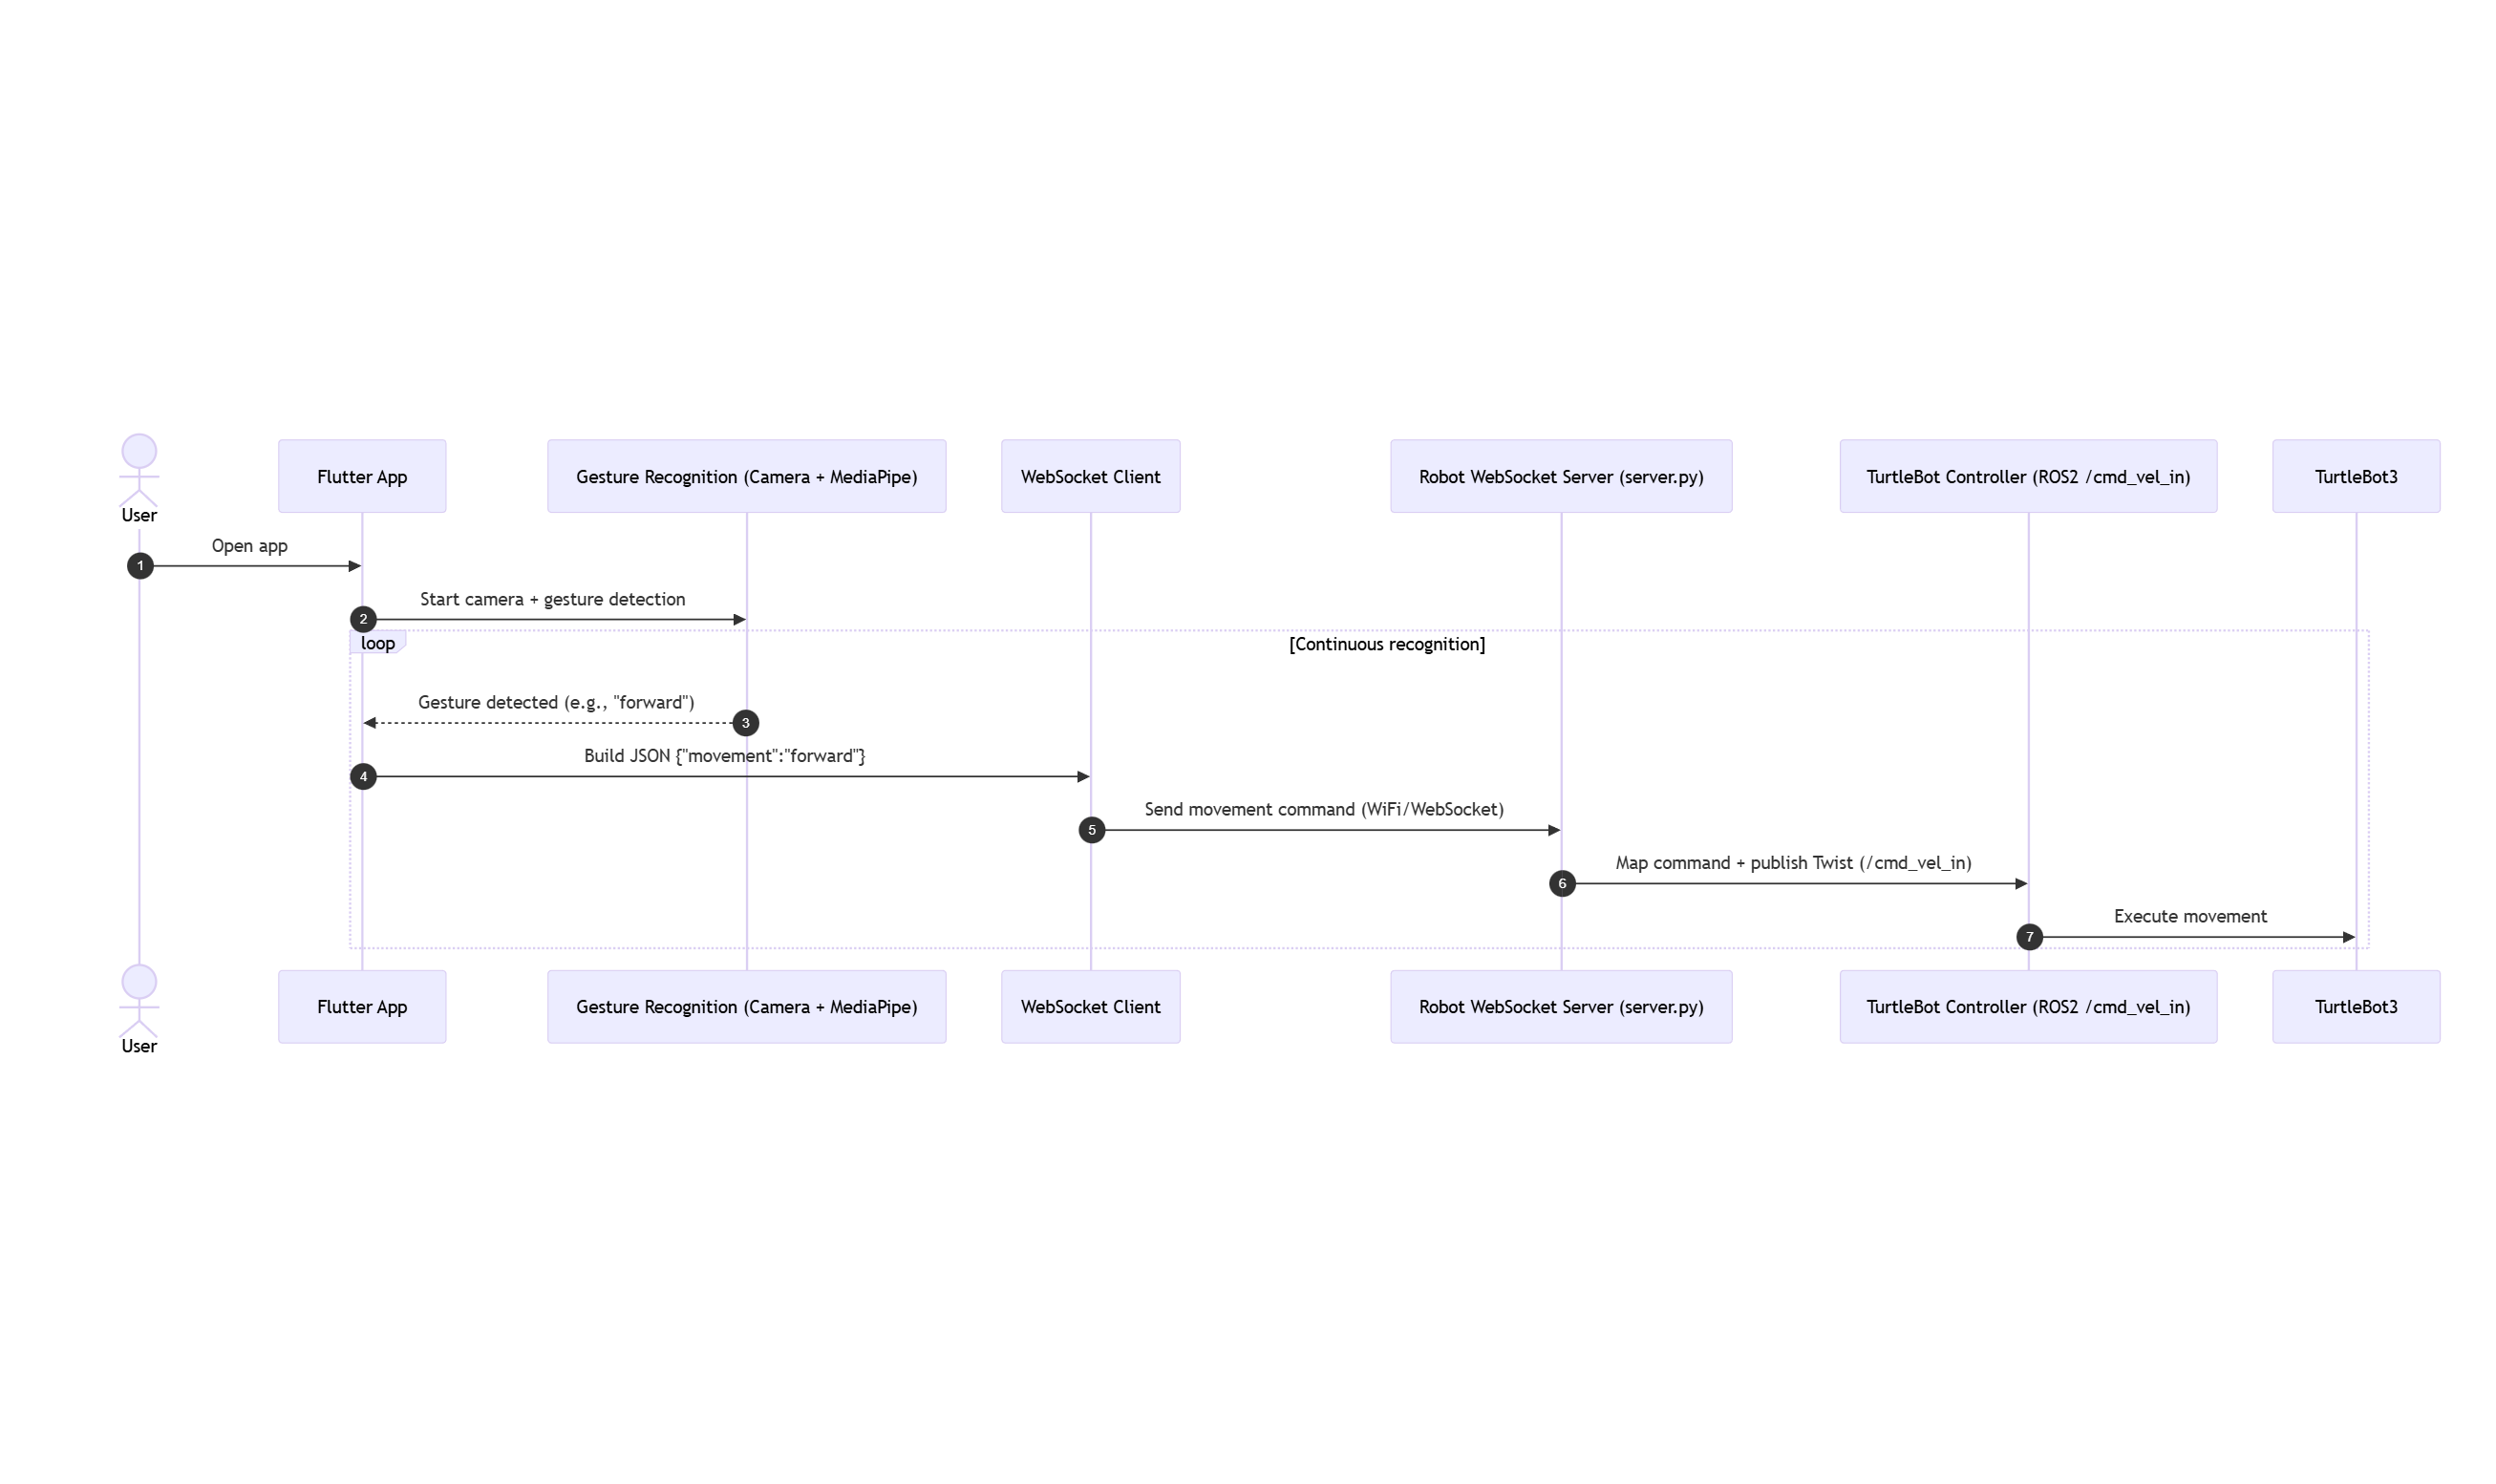
\includegraphics[width=1\textwidth]{figures/use_case_diagram_placeholder.png}
    \caption{External Sequence Diagram}
\end{figure}



\newpage
\subsection{Scenario 2: Bluetooth WiFi Setup (Provisioning)}
\textbf{Goal:} The user configures WiFi on the TurtleBot via Bluetooth, so that the app can connect via WiFi afterwards.

\textbf{Actors:} User, Mobile App, TurtleBot, Bluetooth, WiFi Network

\textbf{Basic Flow:}
\begin{enumerate}[leftmargin=1.5cm]
    \item User opens the Bluetooth WiFi Setup screen in the app.
    \item The app scans for nearby Bluetooth devices.
    \item The user selects the TurtleBot provisioning device.
    \item The app sends WiFi credentials (SSID + password).
    \item The TurtleBot connects to the WiFi network.
    \item The TurtleBot sends back connection status updates.
    \item The TurtleBot sends its assigned IP address to the app.
    \item The app saves the IP and switches to WiFi communication.
\end{enumerate}

\begin{figure}[H]
    \centering
    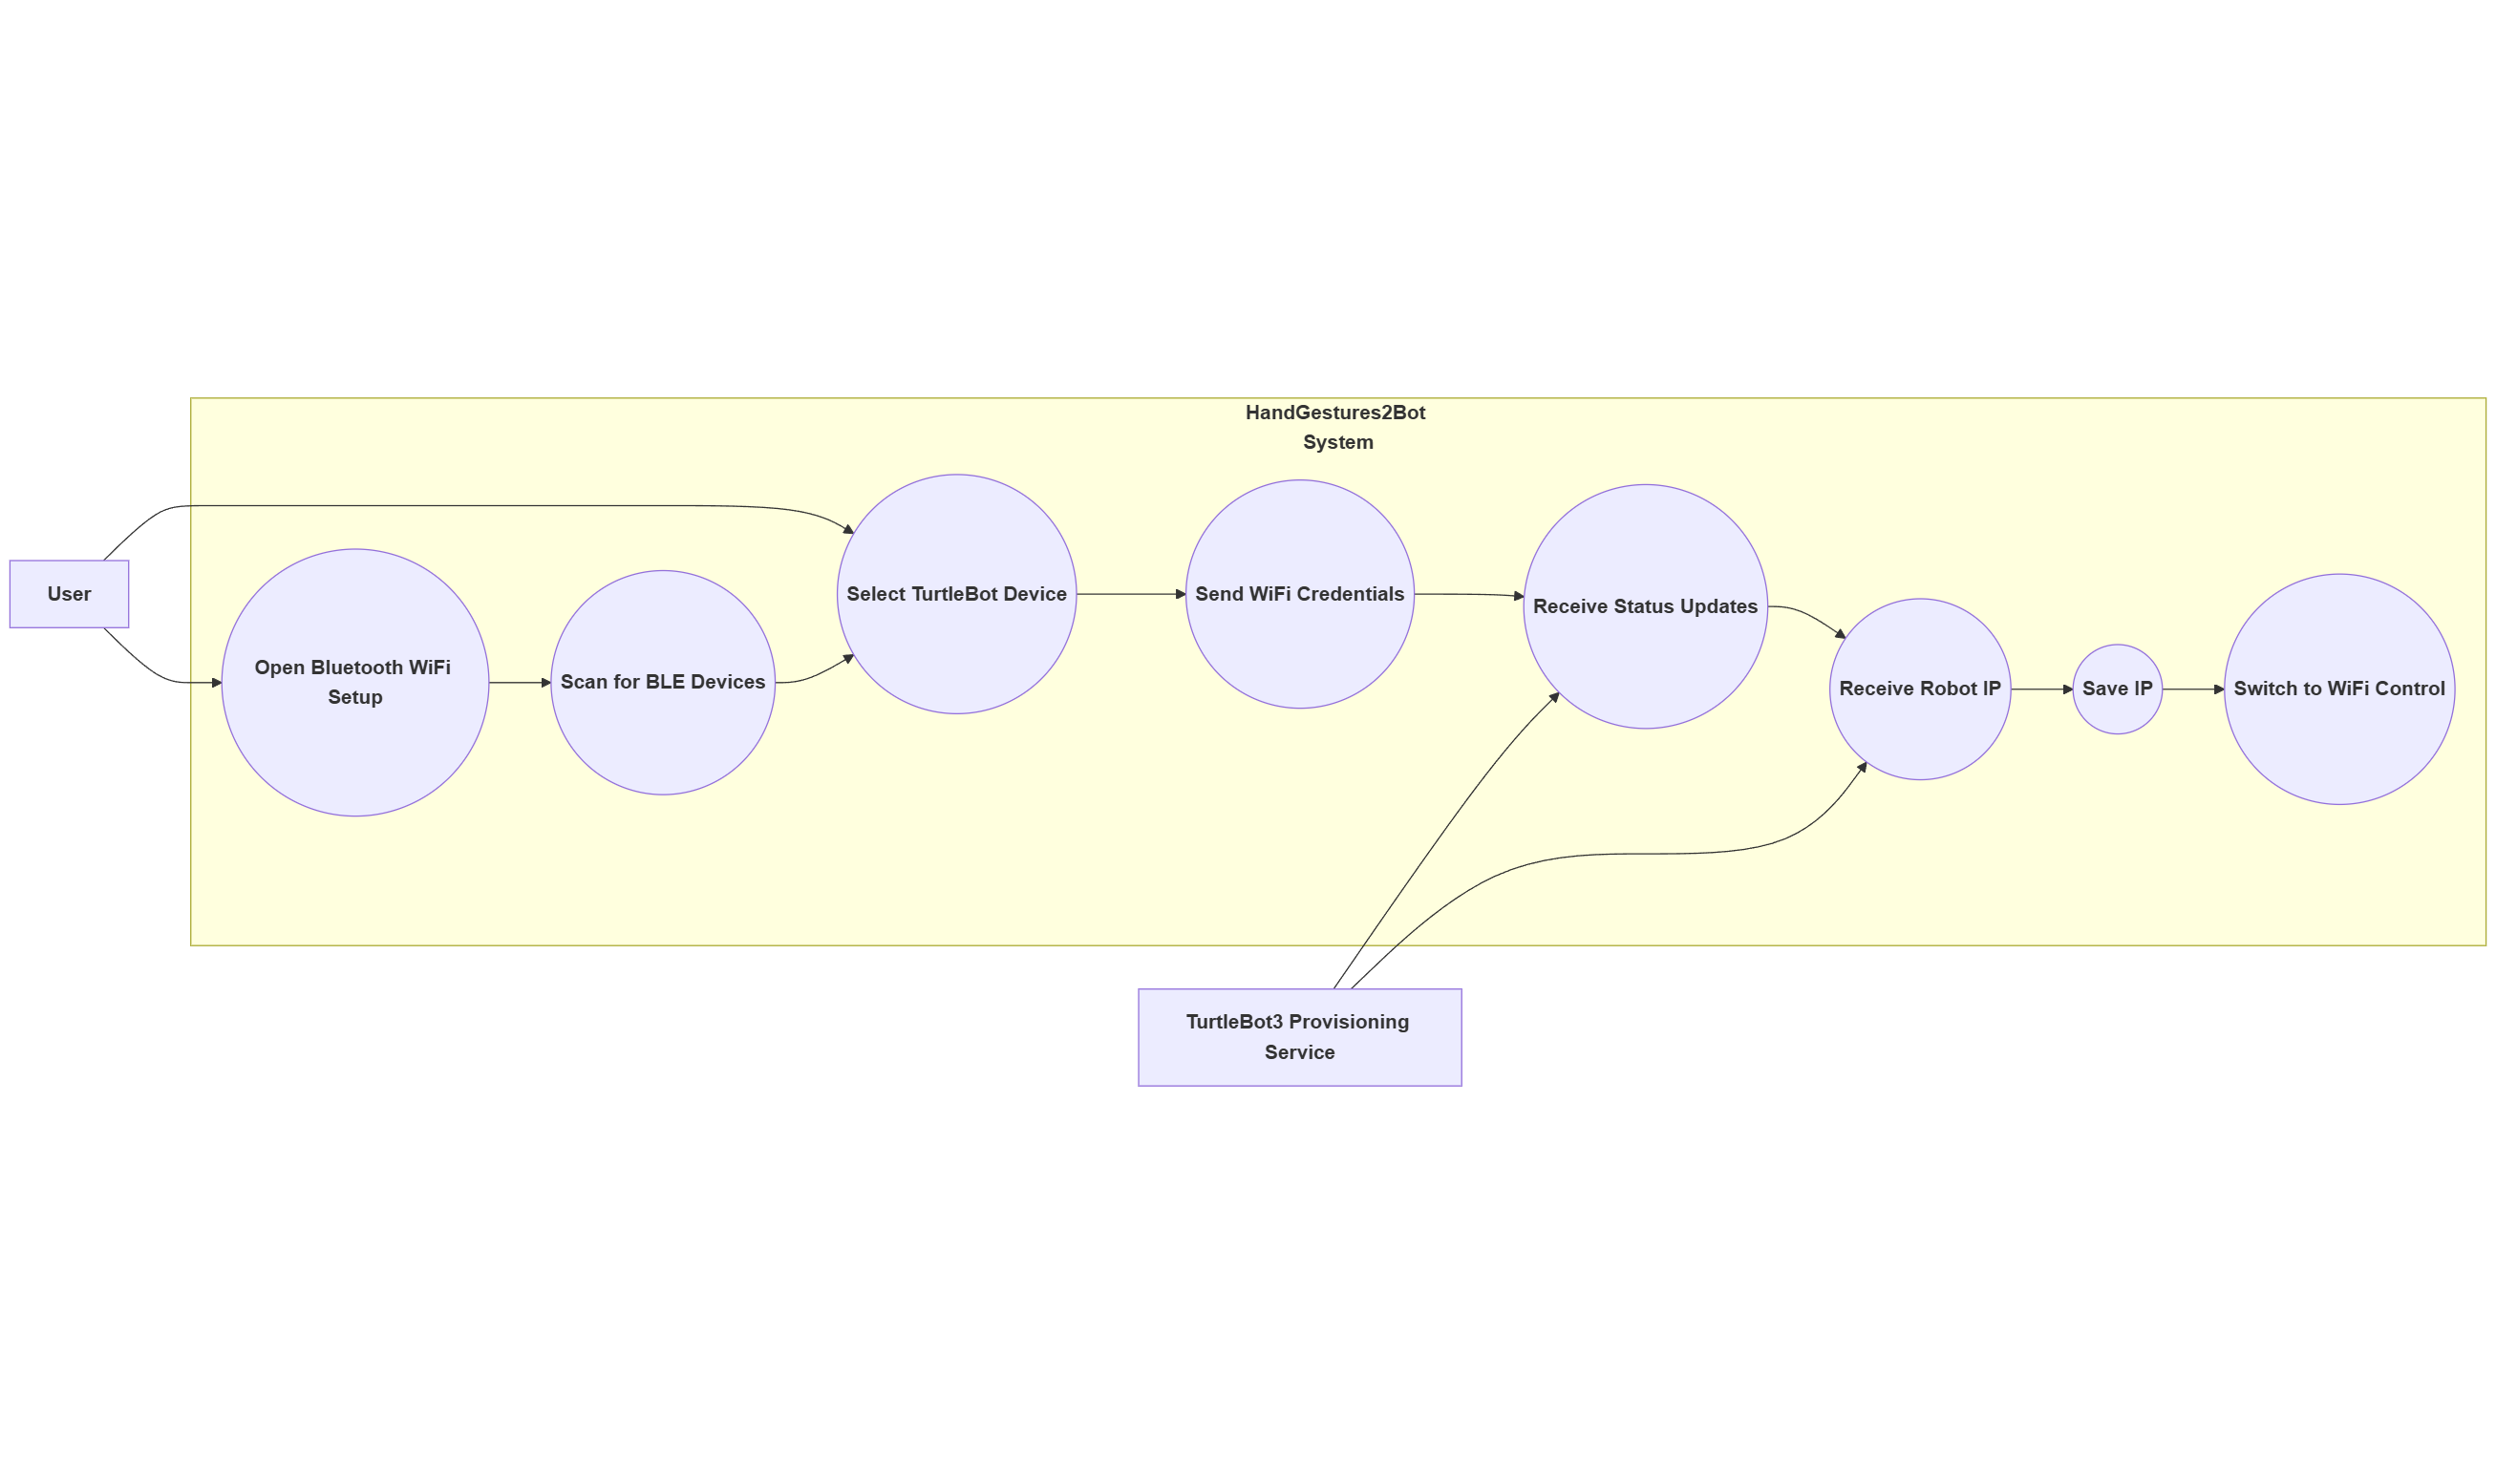
\includegraphics[width=0.95\textwidth]{figures/sequence_external_placeholder.png}
    \caption{Use Case Diagramm (App $\leftrightarrow$ Robot via Bluetooth/WiFi)}
\end{figure}



\newpage
\subsection{UI / Wireframes (No screenshots here)}
\begin{figure}[H]
    \centering
    
\includegraphics[width=0.9\textwidth]{figures/wireframe_placeholder.png}
    \caption{Wireframe Placeholder -- Bluetooth Setup and Gesture Control}
\end{figure}

% =================================================
% 4. ARCHITECTURE (INTERNAL)
% =================================================
\section{Architecture (Internal)}

This section describes the internal structure and interactions of the system.
It includes static and dynamic views of internal components.

\subsection{Static View (Components / Packages)}
The system consists of multiple major parts:

\begin{itemize}[leftmargin=1.5cm]
	\item \textbf{Flutter Mobile App (Dart):} Main user interface and control logic.
	\item \textbf{Gesture Recognition (MediaPipe):} Real-time hand tracking via native camera pipeline.
	\item \textbf{Voice Control:} Speech-to-text and AI-based command parsing.
	\item \textbf{Bluetooth Wi-Fi Provisioning (BLE):} Wi-Fi setup via Bluetooth Low Energy.
	\item \textbf{WebSocket Communication:} Robot control and status feedback over Wi-Fi.
	\item \textbf{Robot Control (ROS 2):} Velocity publishing and robot movement execution.
	\item \textbf{Safety Layer (LiDAR):} Obstacle detection and motion filtering.
\end{itemize}

\newpage
\subsection{Dynamic View (Key Internal Interactions)}
This section describes the most important runtime interactions between the main components of the system.

\subsubsection{Gesture Control $\rightarrow$ Robot Movement}
\textbf{Goal:} Move the TurtleBot using hand gestures from the mobile app.

\begin{enumerate}[leftmargin=1.5cm]
	\item The native camera pipeline detects a hand gesture (MediaPipe).
	\item The gesture is forwarded to the Flutter app via the gesture MethodChannel.
	\item The Flutter UI maps the gesture to a movement command (e.g., \texttt{forward}).
	\item The app sends a JSON command over WebSocket to the robot.
	\item The robot WebSocket server receives the message and forwards it to the movement handler.
	\item The robot publishes a velocity command to \texttt{/cmd\_vel\_in}.
	\item The safety scanner filters unsafe motion using LiDAR data and publishes safe velocity to \texttt{/cmd\_vel}.
\end{enumerate}

\subsubsection{Obstacle Feedback $\rightarrow$ App Warning Overlay}
\textbf{Goal:} Inform the user when motion is blocked due to obstacles.

\begin{enumerate}[leftmargin=1.5cm]
	\item The safety scanner reads LiDAR scan data from \texttt{/scan}.
	\item It computes obstacle distances and publishes an obstacle status message on \texttt{/obstacle\_status}.
	\item The robot WebSocket server subscribes to \texttt{/obstacle\_status} and broadcasts updates to connected clients.
	\item The mobile app receives the obstacle status via WebSocket.
	\item The UI overlays warnings and blocked-motion indicators in the camera view.
\end{enumerate}

\subsubsection{Bluetooth Wi-Fi Provisioning}
\textbf{Goal:} Configure robot Wi-Fi credentials and obtain the robot IP address.

\begin{enumerate}[leftmargin=1.5cm]
	\item The user opens the Bluetooth Wi-Fi Setup page in the app and starts scanning.
	\item The phone connects to the robot provisioning device via BLE.
	\item The app sends SSID and password to the robot via BLE characteristics.
	\item The robot connects to the Wi-Fi network and updates its provisioning status.
	\item The robot sends status updates and its assigned IP address back to the app.
	\item The app stores the IP locally and uses it for future WebSocket connections.
\end{enumerate}

\subsubsection{Voice Control $\rightarrow$ Robot Movement}
\textbf{Goal:} Move the robot using spoken commands.

\begin{enumerate}[leftmargin=1.5cm]
	\item The user speaks a command in the voice control view.
	\item The app converts speech to text (STT).
	\item The AI service interprets the text and generates a movement command.
	\item The command is sent via WebSocket to the robot (same path as gesture control).
	\item Optional TTS feedback is played to confirm the action.
\end{enumerate}


\begin{figure}[H]
	\centering
	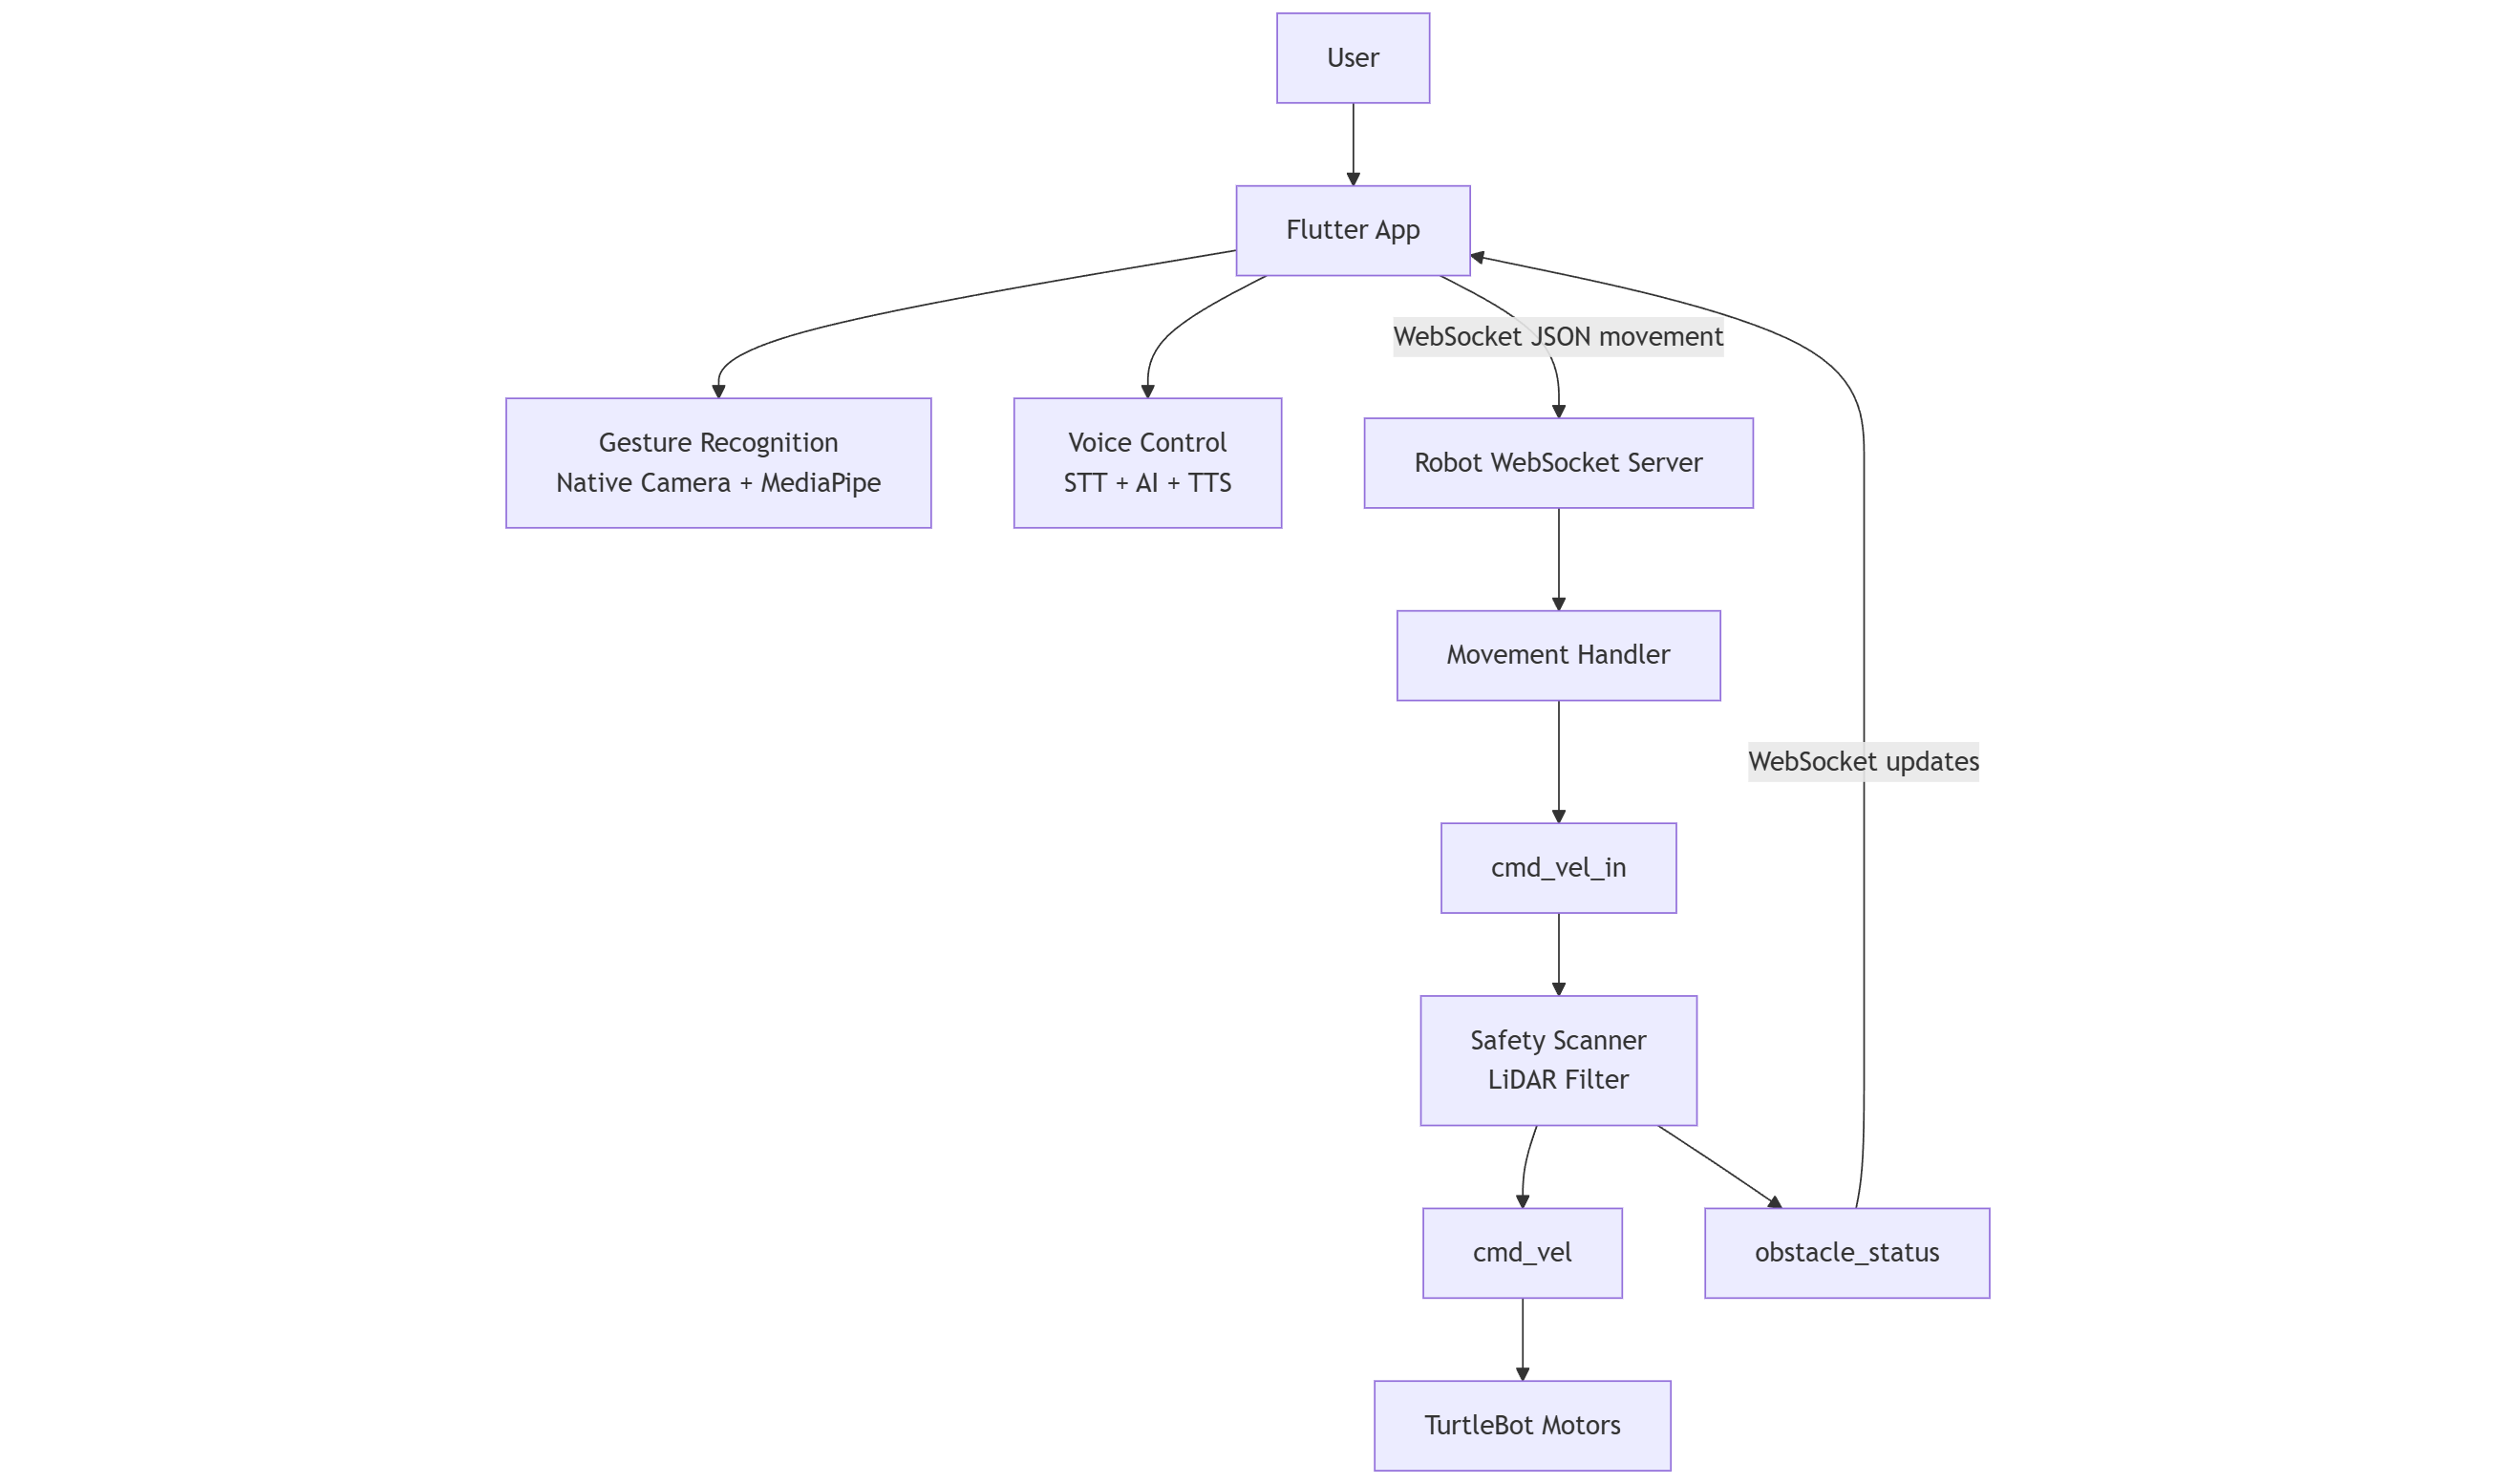
\includegraphics[width=0.9\textwidth]{figures/dynamic_view.png}
	\caption{Flowchart (Data Flow Diagram / System Interaction Flow)}
\end{figure}

% =================================================
% 5. TECHNOLOGIES AND REFERENCES
% =================================================

\newpage
\section{Technologies, Libraries, and References}

This section lists all important technologies, libraries, frameworks, and reused components.
This is necessary to avoid plagiarism assumptions.

\subsection{Technologies Used (excluding iOS)}
\begin{itemize}[leftmargin=1.5cm]
	\item Flutter SDK (Material UI) for the mobile application
	\item WebSocket communication over Wi-Fi for robot control
	\item Bluetooth Low Energy (BLE) for Wi-Fi provisioning
	\item Android CameraX for camera preview and analysis
	\item MediaPipe Tasks Vision for hand landmark detection and gesture recognition
	\item ROS 2 Humble for robot control and messaging
	\item TurtleBot3 platform (real robot and simulation)
\end{itemize}

\subsection{Important Libraries / Frameworks}
\begin{itemize}[leftmargin=1.5cm]
	\item \textbf{Flutter / Dart:} \texttt{web\_socket\_channel}, \texttt{shared\_preferences}, \texttt{speech\_to\_text},
	\texttt{flutter\_tts}, \texttt{http}, \texttt{audioplayers}, \texttt{flutter\_gemma}
	\item \textbf{Android:} CameraX, MediaPipe Tasks Vision, Android BLE GATT stack
	\item \textbf{Robot / ROS 2:} \texttt{rclpy}, standard ROS messages, Python \texttt{websockets}
	\item \textbf{Robot BLE provisioning:} BlueZ / \texttt{bluezero}, \texttt{netifaces}, \texttt{wpa\_cli} / \texttt{nmcli}
\end{itemize}

\subsection{External Services / Assets}
\begin{itemize}[leftmargin=1.5cm]
	\item ElevenLabs Text-to-Speech API (cloud service)
	\item MediaPipe hand landmark model file (\texttt{hand\_landmarker.task})
\end{itemize}

\subsection{Reused / Preexisting Components}
\begin{itemize}[leftmargin=1.5cm]
	\item TurtleBot3 hardware platform and its base ROS ecosystem
	\item ROS 2 Humble and TurtleBot3 packages (e.g., bringup and Gazebo simulation)
	\item Preinstalled ROS 2 simulation packages on the provided Ubuntu virtual maschine from lab lecture (used for testing and simulation)
	\item MediaPipe framework and pretrained hand landmark model
\end{itemize}


\subsection{Important Implementation Notes (Bluetooth Fix)}
A key issue was that the iOS app received the IP address but did not forward it correctly to Flutter.
This was fixed by connecting iOS callbacks to the Flutter MethodChannel and handling them on the Dart side.

\textbf{Key files involved:}
\begin{itemize}[leftmargin=1.5cm]
    \item \texttt{AppDelegate.swift}
    \item \texttt{BluetoothProvisioningService.swift}
    \item \texttt{native\_bluetooth\_service.dart}
\end{itemize}

% =================================================
% APPENDIX
% =================================================
\newpage
\appendix
\section{Appendix}

\subsection{Sprint History}
If you have sprint logs, milestones, or GitHub issue history, you can include them here.

\subsection{Screenshots Reference}
Screenshots are stored in a separate \texttt{screenshots/} directory.
In the main document, screenshots are not included to avoid bloating.
Instead, screenshots can be referenced by filename or included here.

\subsection{Additional Diagrams}
Additional diagrams such as detailed sequence diagrams, class diagrams, or extended wireframes may be placed here.

\end{document}
